\section{Czytania}

\begin{itemize}
    \item wszyscy procesyjnie udają się do ołtarza i rozchodzą się na boki (bez
          skłonu)
          \begin{figure}[h]
              \centering
              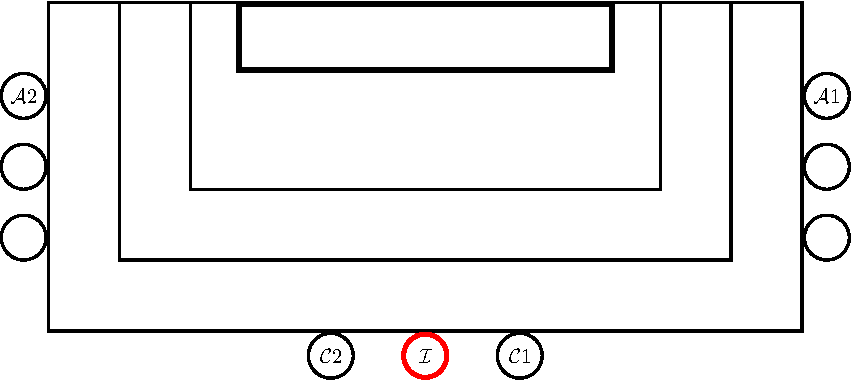
\includegraphics[scale=0.7]{Piatek/Wejscie.pdf}
          \end{figure}
    \item \ii~ wraz z ministrantami wykonują skłon, po czym \ii~ pada na twarz,
          a ministranci klękają na posadzce i skłaniają głowy
    \item \ii~ wraz z \cc1 wstają, a ministranci prostują się i śpiewana jest
          modlitwa
    \item po modlitwie wszyscy powstają, robią skłon i udają się na swoje
          miejsca (\ii, \aa1, \aa2 i \cc~ na sedile)
    \item \cc2 zabiera poduszkę ze stopni ołtarza
    \item \tt~ przynosi pulpit na środek prezbiterium
    \item wszyscy siadają razem z \ii~ i \aa\aa
    \item śpiewana jest lekcja, po niej następuje responsorium i modlitwa
    \item na \textit{Oremus} wszyscy wstają, na \textit{Flectamus genua} -
          klękają, na \textit{Levate} - wstają, po skończonej modlitwie -
          siadają
    \item następuje kolejne czytanie i responsorium
    \item podczas responsorium \cc2 przenosi pulpit na stronę Ewangelii i
          kładzie go na posadzce
    \item po responsorium \ii~ odmawia modlitwę przed stopniami ołtarza po czym
          udaje się do pulpitu i czyta Mękę Pańską
    \item ministranci po jej zakończeniu nie mówią \textit{Laus tibi, Christe}
\end{itemize}